\documentclass[11pt]{article}
\usepackage[utf8]{inputenc}  
\usepackage[T1]{fontenc}
% \usepackage[francais]{babel}
\usepackage{amsmath,textcomp,amssymb,geometry,graphicx,enumerate}
\usepackage{algorithm} % Boxes/formatting around algorithms
\usepackage[noend]{algpseudocode} % Algorithms
\usepackage{titletoc}
\usepackage{hyperref}
\usepackage{stmaryrd}
\usepackage{titling}
\usepackage{amsmath}
\usepackage{stackengine}
\usepackage{multirow}
\usepackage{xcolor}
\usepackage[cache=false]{minted}
\usepackage{mathtools}
\usepackage{boldline}
\usepackage{booktabs}
\usepackage{tikz}
\usepackage[edges]{forest}
\usepackage{gensymb}
\usepackage{enumerate}
\usepackage{pgfplots}
\usepackage{caption}
\usepackage{fancyhdr}
\usepackage{soul}
\usepackage{varwidth}
\usepackage{multicol}
\usepackage{color, colortbl}
\PassOptionsToPackage{table,dvipsnames}{xcolor}
% \usepackage[table, dvipsnames]{xcolor}
\usetikzlibrary{tikzmark,calc,fit}

\newcommand{\hlc}[2][gray]{{%
    \colorlet{foo}{#1}%
    \texttt{\sethlcolor{foo}\hl{#2}}}%
}

\dottedcontents{section}[1.5em]{}{1.7em}{0.7pc}


\definecolor{folderbg}{RGB}{124,166,198}
\definecolor{folderborder}{RGB}{110,144,169}

\newlength\Size
\setlength\Size{4pt}
\tikzset{%
  folder/.pic={%
    \filldraw [draw=folderborder, top color=folderbg!50, bottom color=folderbg] (-1.05*\Size,0.2\Size+5pt) rectangle ++(.75*\Size,-0.2\Size-5pt);
    \filldraw [draw=folderborder, top color=folderbg!50, bottom color=folderbg] (-1.15*\Size,-\Size) rectangle (1.15*\Size,\Size);
  },
  file/.pic={%
    \filldraw [draw=folderborder, top color=folderbg!5, bottom color=folderbg!10] (-\Size,.4*\Size+5pt) coordinate (a) |- (\Size,-1.2*\Size) coordinate (b) -- ++(0,1.6*\Size) coordinate (c) -- ++(-5pt,5pt) coordinate (d) -- cycle (d) |- (c) ;
  },
}
\forestset{%
  declare autowrapped toks={pic me}{},
  pic dir tree/.style={%
    for tree={%
      folder,
      font=\ttfamily,
      grow'=0,
    },
    before typesetting nodes={%
      for tree={%
        edge label+/.option={pic me},
      },
    },
  },
  pic me set/.code n args=2{%
    \forestset{%
      #1/.style={%
        inner xsep=2\Size,
        pic me={pic {#2}},
      }
    }
  },
  pic me set={directory}{folder},
  pic me set={file}{file},
}


\def \Subject {Natural Language Processing}
\def \Course {Final Project\\\small Final Phase}
\def \Author {Alireza Moradi}
\def \Report {Summer 2021}
\def \Prof {Sauleh Eetemadi}
\def \StudentNumber {96521479}

\newcommand\xrowht[2][0]{\addstackgap[.5\dimexpr#2\relax]{\vphantom{#1}}}
\hypersetup{
    colorlinks=true,
    linkcolor=blue,
    filecolor=magenta,      
    urlcolor=blue,
    linktoc = all,
}


% \setminted{
%     frame=lines,
%     framesep=2mm,
%     baselinestretch=1.0,
%     xrightmargin=0in,
%     xleftmargin=0in,
%     fontsize=\footnotesize,
%     linenos=false
% }


\def\Name{\textbf{Alireza Moradi}}  % Your name
\def\SID{Lycée Lakanal}
\def\Login{Classe de PCSIa} % Your login (your class account, cs170-xy)
\def\Homework{2} % Number of Homework
\def\Session{}

\definecolor{LightGray}{gray}{0.925}

% \title{\textbf{NLP}\\Final Project\\\small Phase 2}
\title{
    \includegraphics[width=0.5\linewidth]{../reports/IUST_logo_color.png} \\
    \textbf{Department of Computer Engineering}\\
}
% \author{\Name}

% \markboth{\Session\   \Name}{\Session\  \Name, \texttt{\Login}}
% \pagestyle{myheadings}


\newenvironment{qparts}{\begin{enumerate}[{(}a{)}]}{\end{enumerate}}
\def\endproofmark{$\Box$}
\newenvironment{proof}{\par{\bf Proof}:}{\endproofmark\smallskip}

\textheight=9in
\textwidth=6.5in
\topmargin=-.75in
\oddsidemargin=0.25in
\evensidemargin=0.25in

\newcommand\xDownarrow[1][2ex]{%
   \mathrel{\rotatebox{90}{$\Leftarrow{\rule{#1}{0pt}}$}}
}

\begin{document}
\date{\vspace{-15pt}}
\maketitle

\thispagestyle{empty}
\begin{center}
\vspace{.4cm}
{\bf {\huge \Subject}}\\
\vspace{2pt}
{\bf \Large \Course\footnote{\texttt{https://github.com/Alireza1044/cs224n-final-project}}}
\vspace{.2cm}
\end{center}
{\bf \Author } 
\hspace{\fill} 
{Prof. \Prof} \\
{\bf Student No.:\ \StudentNumber}
\hspace{\fill} 
{\small \Report} \\
\hrule
\vspace{0.8cm}

\clearpage
\setcounter{page}{1}
\pagenumbering{roman}

\tableofcontents
\newpage
\listoffigures
\addcontentsline{toc}{section}{\listfigurename}
\listoftables
\addcontentsline{toc}{section}{\listtablename}

\clearpage
\pagenumbering{arabic}

\newcolumntype{g}{>{\columncolor{Gray}}c}
\definecolor{Gray}{gray}{0.9}
\definecolor{DarkGray}{gray}{0.65}


\section{Word2vec}
The results in figure \ref{fig:michael_word2vec} and \ref{fig:dwight_word2vec} are for 25 of common words between the two classes. The loss at the end of training was around 5.5 . The word \textit{scranton} has a similar vector in both classes which makes sense because their work place is located at Scranton, PA and this word is usually used in the same context with pretty similar neighboring words. The word \textit{hello} has two completely different vectors, and that is justifiable because one of the characters has a sarcastic behavior and several times during the series he uses this word in a sarcastic manner:)

\begin{figure}[H]
    \centering
    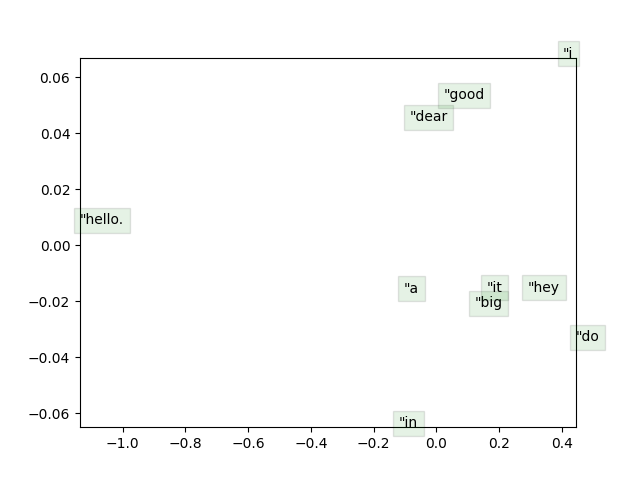
\includegraphics[scale=0.65]{reports/word_vectors_michael.png}
    \caption{First class word vectors}
    \label{fig:michael_word2vec}
\end{figure}

\begin{figure}[H]
    \centering
    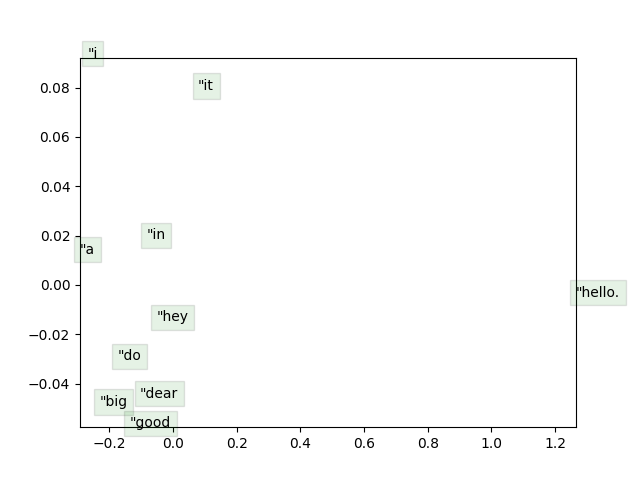
\includegraphics[scale=0.65]{reports/word_vectors_dwight.png}
    \caption{Second class word vectors}
    \label{fig:dwight_word2vec}
\end{figure}

\section{Tokenization}

\begin{table}[H]
    \centering
    \begin{tabular}{|c|c|c|c|}
    \hline
        Vocab Size & Iteration & <UNK> \% & Average \\ \hline
         \multirow{5}{*}{50} & 1 & 0.046 & \multirow{5}{*}{0.045} \\ \cline{2-3}
         & 2 & 0.047 & \\ \cline{2-3}
         & 3 & 0.028 & \\ \cline{2-3}
         & 4 & 0.048 & \\ \cline{2-3}
         & 5 & 0.055 & \\ \hline
         \multirow{5}{*}{150} & 1 & 0.076 & \multirow{5}{*}{0.070} \\ \cline{2-3}
         & 2 & 0.074 & \\ \cline{2-3}
         & 3 & 0.078 & \\ \cline{2-3}
         & 4 & 0.078 & \\ \cline{2-3}
         & 5 & 0.047 & \\ \hline
         \multirow{5}{*}{500} & 1 & 0.073 & \multirow{5}{*}{0.097} \\ \cline{2-3}
         & 2 & 0.0110 & \\ \cline{2-3}
         & 3 & 0.074 & \\ \cline{2-3}
         & 4 & 0.12 & \\ \cline{2-3}
         & 5 & 0.11 & \\ \hline
         \multirow{5}{*}{1000} & 1 & 0.123 & \multirow{5}{*}{0.128} \\ \cline{2-3}
         & 2 & 0.124 & \\ \cline{2-3}
         & 3 & 0.143 & \\ \cline{2-3}
         & 4 & 0.143 & \\ \cline{2-3}
         & 5 & 0.11 & \\ \hline
         \multirow{5}{*}{1500} & 1 & 0.110 & \multirow{5}{*}{0.130} \\ \cline{2-3}
         & 2 & 0.150 & \\ \cline{2-3}
         & 3 & 0.12 & \\ \cline{2-3}
         & 4 & 0.14 & \\ \cline{2-3}
         & 5 & 0.13 & \\ \hline
    \end{tabular}
    \caption{<UNK> token percentage grouped by vocab size}
    \label{tab:unk}
\end{table}

As it can be seen from the data in table \ref{tab:unk}, using vocab size 50 produces the best results.

\section{Parsing}

The model was trained on the original data for assignment 3. Below are 10 sentences from my own dataset which were parsed by the model. The UAS score on these samples was 86.81\%. The model performs well (UAS 100\%) on short sentences or sentences that are only a single part (e.g. have only one verb and no , in the middle of the sentence). On long sentences or complex sentences, the model struggles. I believe this problem can be fixed with more training data.

\begin{enumerate}
    \item \textbf{your quarterlies look very good.} \newline [(2, 1), (3, 2), (5, 4), (3, 5), (3, 6), (0, 3)]
    \item \textbf{how are things at the library?} \newline [(3, 2), (3, 1), (6, 5), (6, 4), (3, 6), (3, 7), (0, 3)]
    \item \textbf{you are a gentleman and a scholar.} \newline [(4, 3), (4, 2), (4, 1), (4, 5), (7, 6), (4, 7), (4, 8), (0, 4)]
    \item \textbf{so this is my kingdom, as far as the eye can see.} \newline [(5, 4), (5, 3), (5, 2), (5, 1), (5, 6), (8, 7), (11, 10), (13, 12), (13, 11), (13, 9), (8, 13), (5, 8), (5, 14), (0, 5)] 
    \item \textbf{you are going to be my accomplice.} \newline [(3, 2), (3, 1), (7, 6), (7, 5), (7, 4), (3, 7), (3, 8), (0, 3)]
    \item \textbf{i think the conference room should be fine.} \newline [(2, 1), (5, 4), (5, 3), (8, 7), (8, 6), (8, 5), (2, 8), (2, 9), (0, 2)]
    \item \textbf{i slashed benefits to the bone.} \newline [(2, 1), (6, 5), (6, 4), (3, 6), (2, 3), (2, 7), (0, 2)]
    \item \textbf{the employees went crazy, i got no help from corporate.} \newline [(2, 1), (3, 2), (3, 4), (7, 6), (7, 5), (7, 3), (9, 8), (11, 10), (9, 11), (7, 9), (7, 12), (0, 7)]
    \item \textbf{if you do not raise your hand, it will not be covered.} \newline [(5, 4), (5, 3), (5, 2), (5, 1), (7, 6), (5, 7), (13, 12), (13, 11), (13, 10), (13, 9), (13, 8), (13, 5), (13, 14), (0, 13)]
    \item \textbf{you have forfeited that privilege.} \newline [(3, 2), (3, 1), (5, 4), (3, 5), (3, 6), (0, 3)]
\end{enumerate}

\section{Language Model}

\begin{table}[H]
    \centering
    \begin{tabular}{|c|c|}
    \hline
         \multirow{3}{*}{Michael} & the office examination, perfect try. is, come breakfast. oh, what is the \\ \cline{2-2}
         & corporate is stay very acupuncture, minority. it is not not to start
 \\ \cline{2-2}
         & they want us to youtube? john copy, delivery for win. here you manage. did \\ \specialrule{2.5pt}{1pt}{1pt}
        \multirow{3}{*}{Dwight} & the office is string with between hunter. i am an little traditional cake \\ \cline{2-2}
         & corporate is way! instructions that is michael! enough i should sailed. coolio.
 \\ \cline{2-2}
         & they want us to once, of my bullet oh, oscar chop you smell him \\ \hline
    \end{tabular}
    \caption{Generated text samples}
    \label{tab:my_label}
\end{table}

The model is a simple LSTM Language Model which was trained for 5 epochs for each of the classes. As it can be seen, sentences generated by the model don't make sense and most of them are also grammatically incorrect (pre-training on a large corpus would be helpful to overcome these problems). On the other hand, generated sentences show some characteristics of the characters which indicates that [much] more training data can improve this.

\section{Fine-Tuning}


\begin{table}[H]
    \centering
    \begin{tabular}{|c|c|}
    \hline
         \multirow{3}{*}{Michael} & i am very happy!pam has a good job.i know. \\ \cline{2-2}
         & i wanted to sit in that bathroom because she was kind of a jerk. \\ \cline{2-2}
         & warehouse has a great, fantastic, very nice office. \\ \specialrule{2.5pt}{1pt}{1pt}
        \multirow{3}{*}{Dwight} & i have to be on vacation with my friend in order to get some cookies. \\ \cline{2-2}
         & i am assistant regional manager.no.no, you are the scranton branch manager.
 \\ \cline{2-2}
         & my farm is an island of passion, fun and hope. \\ \hline
    \end{tabular}
    \caption{Generated text samples}
    \label{tab:my_label}
\end{table}

Generated sentences after fine-tuning are in most cases grammatically correct. They also represent a better characteristics of the speaker. This is because we have a much more complex network (GPT-2) which was also pre-trained on a huge corpus. Despite producing better outputs, we still need more data to have satisfactory outputs in the end.

% \begin{forest}
%   pic dir tree,
%   where level=0{}{% folder icons by default; override using file for file icons
%     directory,
%   },
%     [root
%         [data
%             [raw
%                 [all\_characters
%                     [all\_characters.json, file]
%                 ]
%                 [michael\_dwight\_dialogues
%                     [dwight.txt, file]
%                     [michael.txt, file]
%                 ]
%             ]
%             [clean
%                 [cleaned\_broken\_sentences
%                     [dwight.txt, file]
%                     [michael.txt, file]
%                 ]
%                 [cleaned\_lemmatized\_broken\_sentences
%                     [dwight.txt, file]
%                     [michael.txt, file]
%                 ]
%             ]
%         ]
%     ]
% \end{forest}




% \begin{minted}[
% frame=lines,
% framesep=2mm,
% baselinestretch=1.2,
% bgcolor=LightGray,
% fontsize=\footnotesize,t
% linenos
% ]{python}

% \end{minted}

\end{document}

